\documentclass[a4paper,10pt]{article}
\usepackage{libertine}
\usepackage[utf8x]{inputenc}
\usepackage[T1]{fontenc}

\usepackage[french]{babel}
\usepackage[autolanguage]{numprint}
\usepackage{amsmath}
\usepackage{xcolor}
\usepackage{graphicx}
\usepackage{hyperref}
\usepackage{float}
\graphicspath{{./img/}}
\DeclareGraphicsExtensions{.png, .jpeg, .jpg}
\renewcommand*\thesection{\arabic{section}}
\hypersetup{
    colorlinks,
    citecolor=blue,
    filecolor=blue,
    linkcolor=blue,
    urlcolor=blue
}

\usepackage{geometry}
%\geometry{scale=0.82, nohead}
\usepackage{listings}
\usepackage{caption}
\usepackage{subcaption}
\lstset{keywordstyle=\color{blue}}
\lstset{stringstyle=\color{brown}}
\lstset{showspaces=false}
\lstset{showtabs=false}
\lstset{extendedchars=true}
\lstset{columns=flexible}
\lstset{keepspaces=true}
\lstset{numbers=left, numberstyle=\tiny, stepnumber=1, numbersep=5pt}


\usepackage{tikz}

\title{Calcul efficace des plus longs préfixes communs}
\author{Rémi \textsc{Bois} et Loïc \textsc{Jankowiak}}
\date{\today}
\begin{document}

\maketitle


\section{Introduction}
\label{sec:intro}

L'article de Toru Kasai et al \cite{Kasai01} présente une méthode efficace pour
obtenir les plus longs préfixes communs nécessaires à une recherche
efficace dans un texte. Cette information, d'habitude calculée lors de
la construction du tableau des suffixes, peut dans certaines
applications être absente. L'algorithme présenté par les auteurs
permet alors de retrouver cette information en temps linéaire.


\subsection{Contexte}
\label{sec:context}

Alors que de plus en plus d'applications utilisent de grandes
quantités de données, il est plus que jamais utile d'améliorer les
algorithmes de recherche de motif dans un potentiellement très large
corpus. Les algorithmes à base d'index, comme les arbres des suffixes
et les tableaux des suffixes, permettent d'obtenir de très bons
résultats au prix d'un encombrement mémoire légèrement plus important
(il faut stocker l'index).

Pour ces algorithmes à base d'index, on a besoin de deux structures
pour avoir une recherche efficace en $O(m+ log(n))$, où m est la
taille du motif recherché et n la taille du texte : le tableau ou
l'arbre des suffixes ainsi qu'un tableau comportant des informations
sur les Longest Common Prefixes (lcp) de ces suffixes. Ce second
tableau est généralement créé en même temps que le tableau ou l'arbre des
suffixes, sans occasionner de coût en complexité supplémentaire.

Si l'arbre des suffixes est très efficace pour la recherche de motif,
il occupe beaucoup de place en mémoire. Le tableau des suffixes
adresse ce problème en réduisant la taille d'un facteur 4.

Les algorithmes à base d'index sont très utilisés, notamment en
bioinformatique, où les ``textes'' (des séquences du génome) dans
lesquels les ``motifs'' (une suite de protéines, de bases, ...) sont
recherchés sont très grands. Ces algorithmes sont par exemple utilisés
pour de l'alignement de génomes \cite{Kurtz04}. On peut trouver une
liste des applications dans le papier de Bieganski et al \cite{Bieganski94}.


\subsection{Intérêt}
\label{sec:interest}


L'absence des lcp amène une complexité de recherche de $O(m*log(n))$
au lieu de $O(m+log(n))$. Or, dans certaines applications, cette
information manque. C'est notamment le cas lors d'une compression
Block Sorting, lors de laquelle on peut aisément récupérer un tableau
des suffixes, sans pour autant avoir à disposition les informations
sur les lcp.

Il est alors très utile d'avoir à disposition un algorithme permettant
de retrouver efficacement les informations manquantes. C'est le cas de
celui présenté ici, qui permet de retrouver en $O(n)$ les lcp à
partir du tableau des suffixes. Deux applications utilisant cet
algorithmes sont ensuite présentées : la recherche de motif dans un
texte compressé en Block Sorting et la simulation d'un parcours bottom
up de l'arbre des suffixes.


\section{Une structure permettant de retrouver les \textit{lcp}s}
\label{sec:heightstruct}



\subsection{Le tableau Height}
\label{sec:struct}


% idée : on itère sur les suffixes dans l'ordre d'indice
% et on calcule le lcp avec le précédent dans Pos (ordre lexicographique)
L'idée est la suivante~: plutôt que d'itérer sur le tableau trié
par ordre lexicographique, on choisit d'itérer sur les rangs (les indices de
début des suffixes dans le texte).
Cela permet de réduire le nombre de calculs pour trouver les \textit{lcp}.

Cette réduction s'explique par les trois propriétés suivantes~:


% 3 propriétés :
% - le lcp de 2 sous-chaînes est le minimum des lcp de toutes les sous-chaînes
%   adjacentes dans l'intervalle
\begin{itemize}
\item Le \textit{lcp} de deux sous-chaînes est le minimum des \textit{lcp} de
toutes les sous-chaînes adjacentes de l'intervalle dans le tableau
\textit{Pos}. % expliquer


% - lorsque l'on supprime le premier caractère du suffixe (ie. lorsque l'on
%   avance d'un caractère), l'ordre des suffixes comparés est conservé dans Pos
\item Lorsque l'on supprime le premier caractère du suffixe (ie. lorsque l'on
avance d'un caractère), l'ordre des suffixes comparés est conservé dans
\textit{Pos}.


% - lorsque l'on avance d'un caractère, le lcp diminue de 1 :
%   lcp(A_{Pos[x−1]+1}, A_{Pos[x]+1}) = lcp(A_{Pos[x−1]}, A_{Pos[x]}) - 1.
\item Lorsque l'on avance d'un caractère, le \textit{lcp} diminue de 1 si le lcp
précédent était $\geq$ 1.
\end{itemize}

\subsection{L'algorithme}
\label{sec:algo}

\begin{figure}[h]
  GetHeight\\
  Entrée: Une chaîne A et son tableau des suffixes\\ \hfill \\
  \begin{tabular}{r|l}
    \texttt{1}  & \verb!pour i de 1 à n faire!\\
    \texttt{2}  & \verb!  Rank[Pos[i]] ← i!\\
    \texttt{3}  & \verb!fin pour!\\
    \texttt{4}  & \verb!h ← 0!\\
    \texttt{5}  & \verb!pour i de 1 à n faire!\\
    \texttt{6}  & \verb!  si Rank[i] > 1 alors!\\
    \texttt{7}  & \verb!    k ← Pos[Rank[i]-1]!\\
    \texttt{8}  & \verb!    tantque A[i+h] = A[k+h] faire!\\
    \texttt{9}  & \verb!      h ← h+1!\\
    \texttt{10} & \verb!    fin tq!\\
    \texttt{11} & \verb!    Height[Rank[i]] ← h!\\
    \texttt{12} & \verb!    si h > 0 alors h ← h-1 fin si!\\
    \texttt{13} & \verb!  fin si!\\
    \texttt{14} & \verb!fin pour!\\
  \end{tabular}\\
  \caption{Algorithme de calcul des \textit{lcp} en temps linéaire.}
  \label{fig:getheight}
\end{figure}





\section{Applications}
\label{sec:appli}

Nous allons décrire deux applications dans lesquelles la structure
Height est intéressante. 

La première est un algorithme de compression
qui permet, lors de la décompression d'un texte, de récupérer à la
volée le tableau des suffixes. Il ne reste alors plus qu'à calculer
Height pour pouvoir faire des recherches de motifs efficaces sur le
texte extrait.

La seconde est une utilisation de la structure Height pour simuler un
parcours bottom-up de l'arbre des suffixes. Abouelhoda et al ont
montré par le suite que la structure Height permettait de simuler tous
les parcours d'arbre de suffixes \cite{Abouelhoda200453}.

\subsection{La compression Block Sorting}
\label{sec:blocksorting}

La compression Block Sorting est une compression largement répandue
(bzip2) qui s'appuie sur une transformation de Burrows-Wheeler
dont le but est de rapprocher les caractères identiques d'un texte
afin de pouvoir compresser plus efficacement \cite{Burrows94}.

Cette transformation se réalise en effectuant une rotation du texte à
compresser, puis en ordonnant lexicographiquement les rotations. A
partir de ces rotations ordonnées, on obtient un tableau correspondant
à l'ordre dans lequel les rotations ont été réarrangées ainsi qu'une
chaîne de caractères correspondant aux derniers caractères de chaque
rotation après leur arrangement lexicographique. La figure
\ref{fig:burrows} présente un exemple d'application de cet algorithme
sur la chaîne ``abcabbca\$''. 

\begin{figure}
  \centering
  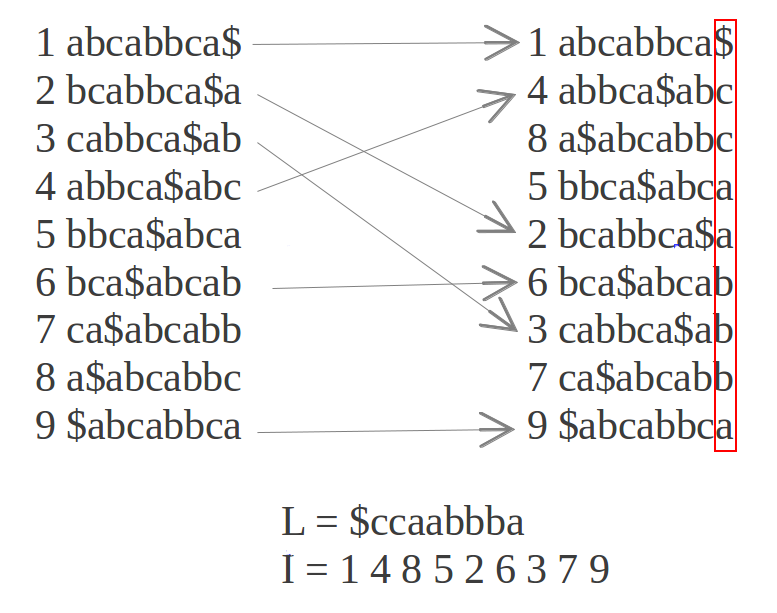
\includegraphics[width=0.5\textwidth]{full_burrows}
  \caption{Application de la transformation de Burrows-Wheeler à la
    chaîne abcabbca\$}
  \label{fig:burrows}
\end{figure}


On remarque que la chaîne obtenue (notée L) est
``\$ccaabbba''. L'objectif de rapprochement des caractères identiques
est bien atteint. Le tableau des indices obtenu (noté I), est
[1,4,8,5,2,6,3,7,9]. A partir de ces deux objets, on peut retrouver le
texte initial. L'efficacité de la compression est dûe au fait qu'une
fois les caractères rapprochés, on peut utiliser un encodage
``move-to-front'', qui consiste, pour chaque caractère, à indiquer sa
distance avec sa prochaine répétition. Cette distance ayant été
raccourcie par la transformation de Burrows-Wheeler, on peut la coder
sur moins de bits. Une fois le ``move-to-front'' effectué, on encode
les caractères via le codage de Huffman, ce qui permet d'optimiser
l'espace mémoire utilisé.

Le tableau I obtenu n'est autre que le tableau des suffixes. En effet,
la rotation, puis ordonnancement par ordre lexicographique revient à
calculer tous les suffixes du textes les uns après les autres, la
seule différence étant que l'algorithme de Burrows-Wheeler ne s'arrête
pas à la fin de la chaîne mais réécrit son début à la suite (ex :
bbca\$abca). La décompression permet de retrouver L et I, puis le
texte à partir de ces deux informations. Lors d'une décompression, on
obtient donc le tableau des suffixes (correspondant à I) sans aucun
coût supplémentaire. Pour faire une recherche efficace, il manque
cependant les informations sur les lcps, que l'on peut obtenir en
calculant le tableau Height tel que décrit section \ref{sec:algo}.


\subsection{Simulation d'un parcours bottom-up}
\label{sec:bottomup}

Un parcours bottom-up consiste à partir de la feuille la plus à gauche
d'un arbre et à remonter à un noeud père uniquement après avoir vu
tous ses fils. Ce type de parcours permet de résoudre de nombreux
problèmes (répétitions en tandem, plus longue sous-chaîne commune,
décomposition de Zip Lempel, ...)\cite{Abouelhoda200453}.

L'article de Kasai et al, présenté en figure \ref{fig:bottomupalgo},
montre qu'on peut, à l'aide du tableau des suffixes et de leur
structure Height, réaliser ce type de parcours en O(n).


\begin{figure}
  \centering
        \begin{tabular}{r|l}
         & Avec Pos tableau des suffixes et Height présenté
         précédemment\\
         \hline
        \texttt{1}  & \verb!S:=(-1,-1); n:=|T| /*Init stack S*/!\\
        \texttt{2}  & \verb!for k:=1 to n+1 do /*k-th stage*/!\\
        \texttt{3}  & \verb! ~(Llca, Hlca) := (k-1, Height[k]);!\\
        \texttt{4}  & \verb! ~(L, H) := top(S);!\\
        \texttt{5}  & \verb! ~while (H > Hlca) do!\\
        \texttt{6}  & \verb! ~ ~(L, H) := pop(S), R := k-1;!\\
        \texttt{7}  & \verb! ~ ~report triple (L, R, H);!\\
        \texttt{8}  & \verb! ~ ~Llca := L;/*Update boundary*/!\\
        \texttt{9}  & \verb! ~ ~(L, H) := top(S);!\\
        \texttt{10} & \verb! ~od!\\
        \texttt{11} & \verb! ~if (H < Hlca) then!\\
        \texttt{12} & \verb! ~ ~Push((Llca,Hlca), S); fi;!\\
        \texttt{13} & \verb! ~Push((k, n - Pos[k] + 1), S);!\\
        \texttt{14} & \verb!od!\\
      \end{tabular}\\
  \caption{L'algorithme de parcours bottom-up}
  \label{fig:bottomupalgo}
\end{figure}

L'algorithme se base sur une pile, remplie au fur et à mesure que l'on
parcoure les feuilles (représentées par le tableau des
suffixes). Lorsque l'on trouve le plus petit ancêtre commun de deux
feuilles (grâce au tableau Height), on ajoute cet ancêtre à la
pile. Il sera retourné lorsque tous ses enfants auront été visités, et
juste avant de retourner le premier enfant du noeud interne suivant.



%décrire les problèmes résolvables par un parcours bottom up de
%l'arbre des suffixes : répétition en tandem, plus longue sous chaîne
%commune, décomposition de Zip Lempel. Citer Abouelhoda pour cette liste.

\section{Conclusion}
\label{sec:conclusion}


Kasai et al proposent un algorithme performant pour calculer les lcps
à partir du tableau des suffixes. Bien que la plupart des applications
calculent les lcps en même temps que le tableau des suffixes, on a pu
voir qu'il existe des cas, comme la décompression d'un texte sous
Burrows-Wheeler, où cette information est manquante.

On a également pu voir que cette structure permettait de simuler des
parcours d'arbre des suffixes.

Enfin, l'espace mémoire requis pour construire les lcps à partir du
tableau des suffixes prend 13n bytes mais peut être ramené à 9n bytes
comme montré par Manzini \cite{Manzini04}.


\bibliographystyle{amsalpha}
\bibliography{./pres.bib}



\end{document}